\documentclass[../../../../../../dd.tex]{subfiles}

\begin{document}

	\subsection{Presentation Tier}
		In this tier, the two main components that are found are the Web Browser User Interface and the Application User Interface. This two components are different in the programming language and they will run on different devices. This two components must comunicate with the controller via the same set of class that must send and read data in the same way. The idea was that the view of the UI can change to be optimized for the device, but the communication with the Logic tier must be the same. So each UI must have two kinds of classes: the first is composed by the classes of visualization, that must follow the organization shown on the mock object of the RASD. For example on the RASD we describe all the pages and all the input form of the two kinds of application. The second one must contain a class that can send messages to the Logic Tier and an another class that can receives its responses. The first class is called CommandSender and the second one ResponseReceiver.

		\begin{figure}[H]
				\centering
				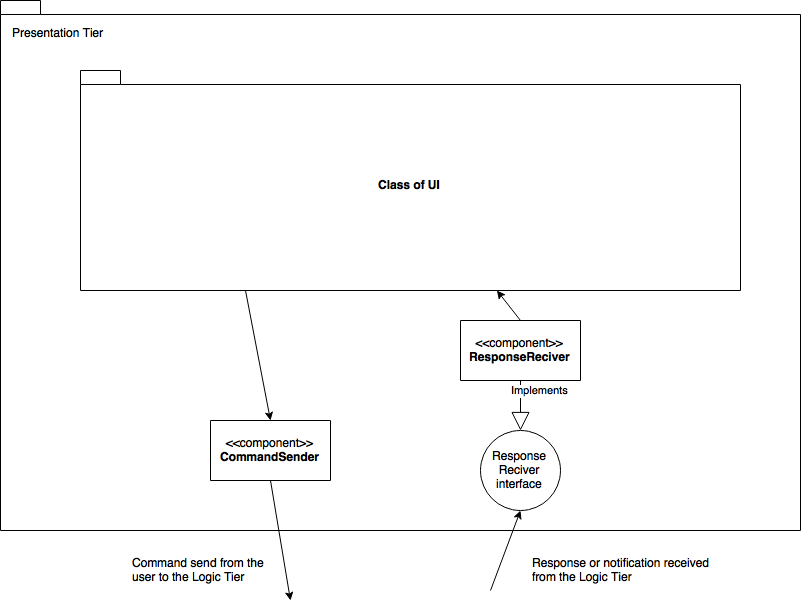
\includegraphics[width=\textwidth, scale=0.5]{../images/PresentationTier.png}
			\caption{Presentation Tier Structure}\label{fig:PresTier}
		\end{figure}
	
\end{document}